\documentclass{IEEEcsmag}

\usepackage[colorlinks,urlcolor=blue,linkcolor=blue,citecolor=blue]{hyperref}
\expandafter\def\expandafter\UrlBreaks\expandafter{\UrlBreaks\do\/\do\*\do\-\do\~\do\'\do\"\do\-}
\usepackage{upmath,color}


\jvol{XX}
\jnum{XX}
\paper{8}
\jmonth{April}
\jname{Publication Name}
\jtitle{Publication Title}
\pubyear{2025}

\newtheorem{theorem}{Theorem}
\newtheorem{lemma}{Lemma}


\setcounter{secnumdepth}{0}

\begin{document}

% Automatyczna aktualizacja modeli w radiologii z wykorzystaniem uczenia ciągłego
\title{Development of AI models in radiology using continuous learning}

\author{Krzysztof Zalewa}
\affil{Wroclaw University of Science and Technology, Wroclaw , Lower Silesia Voivodeship, Poland}

\author{Michał Pakuła}
\affil{Wroclaw University of Science and Technology, Wroclaw , Lower Silesia Voivodeship, Poland}

\markboth{THEME/FEATURE/DEPARTMENT}{THEME/FEATURE/DEPARTMENT}

\begin{abstract}\looseness-0Continuous learning is a method in which the model is dynamically extended to new data and classes.
Therefore, it can be the solution to creating artificial intelligence capable of adapting to an enormous amount of dynamic data and domain changes. 
But the method has its own downsides, from practical problems of storing data, privacy concerns to catastrophic forgetting. 
This article explores recent strategies for using continuous learning and methods alleviating it's weaknesses.
\end{abstract}

\maketitle

\section{INTRODUCTION}
    Machine learning is widely used in many fields of study.
    Machine learning and artificial intelligence (AI) are an everyday topic of studies in a medical setting.
    Medical practices - especially radiology - use a lot of imaging, for example: Magnetic resonance imaging (MRI), X-rays, CT\cite{cite-5}\cite{cite-20}, which generates loads of dynamic clinical data.
    The amount of those images made an urge to create a tool that will constantly analyze and store this data for further use in diagnostics, recognition, or describing.
    Previous generation models like BERT\cite{cite-24} have already achieved high accuracy\cite{cite-24}. 
    However, LLM-based models such as Radiology-GPT or Radiology-Llama2 (based on Chat GPT and LLama, respectively) achieve near-human results \cite{cite-2}\cite{cite-3}. 
    By training artificial intelligence with medical images, these models can provide concise and coherent impressions of the data provided\cite{cite-3}. 
    This can improve the workflow of radiologists and thus improve the quality of care received by patients.

    While using the pre-trained models, we only get the information based on static data that already have been analyzed and verified, but illnesses and humans differ and evolve.
    Often times, reports are so varied that it is difficult even for humans to extract recommendations for further care \cite{cite-25}\cite{cite-9}.
    With heterogeneous data, retraining the AI model every time new data arrive would be impractical.
    Taking into account this fact, researchers have come up with the idea of using Active Learning (AL)\cite{cite-10}\cite{cite-19} and Continuous Learning (CL)\cite{cite-10}\cite{cite-19} or even a combination of both (CAL)\cite{cite-19}.
    The use of these techniques is to aid in clinical decision making\cite{cite-4} and to help understand written reports.
        
    That is why there is a need to update the data set used to analyze imaging results, without human factor, using continual learning.
    Human-side supervision can be limited with the use of self-supervised learning algorithms (SSL)\cite{cite-17}.
    Continuous learning allows AI models to work incrementally, using evolving data and gaining knowledge, without the need to externally verify.
    Although verifying effectiveness of CL approaches is relatively complicated due to types of incremental and replay-based domains.
    Daniel et al.\cite{cite-19} presents a term called IL-Score that is used to compare different models based on given parameters, generalizing its' performance based on assessment of transfer learning, forgetting and capacity of Deep Learning (DL) algorithms.
    Addressing this problem is very important in terms of choosing what practices or parameters to use in each problem.
    
    Given the context, researchers, aware of these challenges, inform us that models using human-in-the-loop algorithms\cite{cite-10} are still crucial to development and are needed to optimize model performance in terms of response accuracy or precise segmentation. 
    
    Regardless of many positive outcomes of studies, continuous learning has its own critical downsides: \linebreak
    1) For the model to have access to previous data, it must be stored.
    That introduces the need for hardware to store these data \cite{cite-1}.\newline
    2) Storage of frequently sensitive medical data can lead to privacy concerns\cite{cite-1}.\newline
    3) With a large amount of data, the problem known as catastrophic forgetting can arise.
    It is a situation where the model forgets previous data and classes.
    Thus, lowering it's performance\cite{cite-1}.\newline
    4) There is distinct lack of standardized datasets and evaluation protocols.
    Which limits ability to train and compare performance of different models\cite{cite-2}\cite{cite-3}.
    
\section{RELATED WORKS}
    \paragraph{Motivations and challenges of Continual Learning in Radiology}
    Most of articles that have been studied have noticed the need to implement continuous learning in radiology to improve the efficiency of a diagnostic process.
    The main motivation is to use an automated process to avoid storing vulnerable data due to privacy restrictions\cite{cite-2}\cite{cite-18}\cite{cite-5}.
    The way data is stored is regulated by the principles of law (standards such as HIPAA)\cite{cite-2}\cite{cite-5}\cite{cite-18}.
    Even if the software is designed to handle the input data properly, the standards may change in the future, and all the collected data will be disqualified due to regulations. 
    
    The solutions presented included anonymization of the data before using it to increment the data available to analyze further images. It requires specialistic algorithms to achieve this task successfully.
    
    Another issue presented can be defined as population variability\cite{cite-20}\cite{cite-11}.
    Due to the rapid growth of life on Earth, there will be even more heterogeneous data to collect programs that use continuous or active learning\cite{cite-11}\cite{cite-20}.
    Generating new data leads to the problem of storage, where (depending on complexity of algorithms) it may not be possible to store all of the labeled data.

    All of these minor issues lead to a major one: \textbf{Catastrophic Forgetting}\cite{cite-18}\cite{cite-10}\cite{cite-1}\cite{cite-17}\cite{cite-19}.
    Addressing this issue is crucial to achieve success in implementing any type of incremental machine learning, especially Continuous Learning.
    Being able to store data safely and increment without forgetting previously learned data is challenging because of how data is written into storage. 
    In articles, researchers have come up with some ideas to prevent it, and it will be discussed further.

    \paragraph{Scenarios and Types of Continual Learning in Medical Imaging}
    Daniel et al. \cite{cite-19} had given a complex explanation about classification in different approaches to adapting models to new context.
    The fundamental scenarios presented were as follows:
    \begin{itemize}
        \item Domain-Incremental Learning (Domain-IL)
        \item Task-Incremental Learning (Task-IL)
        \item Class-Incremental Learning (Class-IL)
    \end{itemize}
    Although these approaches are still increasing security concerns \cite{cite-19}, they are crucial in creating innovative solutions in terms of creating self incrementing tool for radiology.
    Using those scenarios in studies, where static data is used, will give results that will be compared in further studies.

    \paragraph{Overview of Continual Learning Methods} 
    The methodological approaches to continual learning in radiology can be categorized into four main paradigms, each addressing catastrophic forgetting and data variability challenges with distinct strategies:
    
    \textbf{Regularization-based methods} (e.g., EWC \cite{cite-11}, LwF \cite{cite-2}) introduce constraints to preserve critical parameters from previous tasks.
    These techniques use Fisher information matrices (EWC) or knowledge distillation (LwF) to penalize deviations in important weights \cite{cite-11}\cite{cite-5}.
    Doing so allows to contain as much data as needed to address specific task.
    \textit{Strengths}: Privacy-compliant (no raw data storage), lightweight, and suitable for incremental tasks like tumor segmentation \cite{cite-11}\cite{cite-2}.  
    \textit{Limitations}: Performance decay in long-term deployments and rigidity-plasticity trade-offs during domain shifts \cite{cite-11}\cite{cite-17}.  
    
    \textbf{Replay-based methods} retain subsets of past data (rehearsal) or generate synthetic samples (generative replay) for retraining \cite{cite-1}\cite{cite-11}, meaning that there is a data samples locally stored for quick access by model.  
    \textit{Strengths}: Effective for class-incremental scenarios (e.g., rare diseases) and domain shifts from scanner variability \cite{cite-1}\cite{cite-11}.  
    \textit{Limitations}: Privacy risks with raw data storage and computational overhead for generative models \cite{cite-11}\cite{cite-17}.
    
    \textbf{Dynamic model expansion} (e.g., task-specific layers \cite{cite-1}, DynaMMo\cite{cite-17}) allocates new parameters for novel tasks or domains.
    This approach allows to store information safely between various scanners.
    \textit{Strengths}: Robust to abrupt distribution shifts (e.g., new imaging protocols) and scalable for multi-organ segmentation \cite{cite-1}\cite{cite-17}.  
    \textit{Limitations}: Increased model complexity and dependency on task identifiers \cite{cite-11}\cite{cite-17}.
    
    \textbf{Hybrid techniques} combine approaches (e.g., EWC + replay \cite{cite-11}) to balance stability and plasticity.  
    \textit{Strengths}: State-of-the-art performance in federated learning and multimodal integration \cite{cite-11}\cite{cite-2}.
    \textit{Limitations}: Higher implementation complexity and computational costs \cite{cite-17}\cite{cite-11}.
    
    In medical imaging, hybrid frameworks show promise for addressing privacy constraints \cite{cite-11}\cite{cite-2}, while dynamic architectures like DynaMMo \cite{cite-17} optimize resource usage in incremental class learning.
    Replay-based methods remain prevalent despite ethical concerns, underscoring the need for standardized benchmarks \cite{cite-11}\cite{cite-5}.

    \paragraph{Practical Applications of CL in Radiology}
    Continual Learning (CL) has emerged as a critical paradigm for adapting AI support evolving demands in radiology. The case studies presented different approaches with respect to various imaging methods and body parts.
    Key applications were addressing \textbf{automated segmentation}(e.g., abdominal tumors \cite{cite-1}), \textbf{cross-modality adaptation}(e.g., X-ray pre-training with MUSCLE \cite{cite-17}), and \textbf{diagnostic workflow optimization}(e.g., breast MRI \cite{cite-21}).
    Challenges such as data heterogeneity or catastrophic forgetting are addressed with hybrid techniques like replay with coresets \cite{cite-26} or regularization strategies \cite{cite-11}.
    These approaches enable models to incrementally integrate new imaging protocols, patients populations, and disease subtypes without retraining from scratch.
    It is important to address those fluctuating parameters, because of innovative solution in medical fields that are showing up everyday.

    \paragraph{Implementation Challenges and Standardization}
    One of the issues to effectively compare results given by non-dependent studies is \textbf{lack of standardized benchmarks}\cite{cite-18}.
    Many studies use non-public datasets and limit reproducibility by other researchers.
    Simultaneously more complicated datasets are needed for proper testing and development making it impossible to create static dataset for benchmarking Continual Learning models.
    Weibin et al. \cite{cite-19} used own metric called IL-Score as a comparison between his research results, given different parameters for models used.

    Kumar et al.\cite{cite-18} recommend the development of specialized, public CL datasets and accessible code repositories to improve transparency, reproducibility, and progress in the field.
    Doing so would enable researchers to successfully classify their results.
    Possibility to compare models with others, based on benchmarks that are developed with standards, would give a measure how clinically relevant researched models are.
    
    \paragraph{Education and Competencies of Radiologists int the AI Era}
    Embracing technology into the real-life radiology scenarios requires changing how radiologists' competencies are defined and what can be expected from the results of the educational framework.
    Current radiology residency programs should prepare to use AI in everyday tasks by emerging \textbf{five-step framework} which combines didactic lectures, hands-on labs, and expert discussion to improve confidence in AI applications \cite{cite-8}.
    Achieving and developing competency in using those tools requires understanding how AI architecture looks like, how was it prepared for clinical implementation, with acknowledging ethical considerations of this solution.
    
    To prevent reinforcing of bad habits in use of those tools and to give sufficient guidance in terms of effective using AI models organizing hybrid learning methods (e.g., interdisciplinary conferences and vendor demos) should be prioritized for skill retention\cite{cite-8}.
    Post-curriculum surveys reveal a 100\% participant confidence boost in AI knowledge, underscoring the need for annual updates and longitudinal assessments to track competency evolution\cite{cite-8}.

    For specialized tasks such as the creation of protocols, machine learning models trained on metadata streamline the standardization of the MRI / CT protocol and clinical indications, have maintained accuracy and reduced radiologists' workload\cite{cite-16}.
    Models that are capable of doing so leverage iterative reconstruction and sparse data techniques to optimize parameters giving results without compromising diagnostic quality \cite{cite-16}.
    Continuous learning is critical, as AI tools like \textbf{Radiology-Llama2} (a domain-specific LLM) and embedded AI assistants in RIS/PACS require radiologists to adapt to iterative model updates and human-AI collaboration workflows\cite{cite-3}\cite{cite-6}.
    Besides, while using Active learning strategies, such as correcting AI-generated annotations in real-time, support "human-in-the-loop" expretise.
    This practice mitigates crucial problems (like catastrophic forgetting) in adapting continuous learning into medical field, simultaneously keeping an expert supervision\cite{cite-6}.
    Nonetheless, it should be only temporary practice in pursuing autonomous system.
    Alternatively, while using models that have been trained with a decentralized approach called Swarm learning, individual radiologists would have to be prepared to gather their own datasets.
    It requires preparation from medical and educational facilities that will provide sufficient courses for radiologists, that will explain how to properly prepare patient data as a dataset element.
    Those datasets should contain annotations, corrections etc. to share to model weights instead of raw patient data\cite{cite-6}\cite{cite-8}.
    Such prepared data would then be shared for model from various clinical facilities.

    \paragraph{Trends and Future Directions for CL in Radiology}
    Continual learning (CL) is gaining traction in radiology as a solution to evolving clinical demands, enabling AI models to adapt incrementally to new imaging protocols, disease patterns, and scanner technologies without catastrophic forgetting.
    Current trends emphasize \textbf{decentralized frameworks} like swarm learning, which allow multi-institutional collaboration while preserving patient privacy through localized model updates and weight-sharing mechanisms\cite{cite-27}.
    Integration of CL platforms into PACS/RIS systems is streamlining real-time feedback loops, empowering radiologists to refine AI outputs during routine workflows\cite{cite-27}.
    However, challenges persist, including computational costs for high-resolution imaging (e.g., whole-slide histopathology) and biases from institution-specific correction patterns\cite{cite-27}.

    Probably in the future most solutions will pursue \textbf{hybrid CL strategies} that blend rehearsal-based methods (e.g., synthetic data generation) with architectural innovations like dynamic neural networks\cite{cite-27}\cite{cite-18}.
    Creating standardized benchmarking datasets (e.g., MedMNIST) and defining protocols capable of connecting different solutions will be critical for cross-institutional validation \cite{cite-27}.
    Educational initiatives must also evolve, prioritizing solutions using CL modules focused on human-in-the-loop in radiology curricula to train future practitioners in model auditing, bias mitigation and collaborative AI stewardship \cite{cite-28}\cite{cite-29}.
    As CL matures, its success will depend on balancing technical advancements with ethical frameworks that ensure equitable, transparent, and clinically actionable AI evolution.
    
    \section{Review of Applications}
    \textbf{Pseudo labels} As mentioned before problem of catastrophic forgetting is one of the biggest problems in continuous learning.
    One of the solutions to this problem proposed by Zhang et al.\cite{cite-1} is generating pseudo labels for each class.
    The proposed method works by:
    \begin{enumerate}
        \item At each training step t the model has already learned the classes form previous step ($C_{t-1}$)
        \item When learning new data, instead of ignoring previous classes the model generates pseudo labels based on previous predictions ($Y_{t-1}$)
        \item Now the loss function considers both real labels from new data and pseudo labels from old data
    \end{enumerate}
    Therefore, the label for class c ($L^c_t$) can be expressed as:
        \[
            L^c_t =  
            \begin{cases}
                L^c_t & \text{if } c \in C_t - C_{t-1} \\
                \hat{Y}^c_{t-1} & \text{if } c \in C_{t-1}
            \end{cases}
        \]
    \textbf{Image-aware organ-specific heads} Another method of dealing with catastrophic forgetting also proposed by Zhang et al.\cite{cite-1}.
    The particular model used by Zhang et al. (Swin UNETR) has a Softmax layer as the output layer that predicts the probabilities of each class.
    The idea behind image-aware organ-specific heads is to replace that output layer with heads dynamically generated based on images global features.
    Once again the whole method can be expressed as equations :
        \[
            \text{Global feature:} \quad  f = \text{GAP}(E(X)),
        \]
        \[
            \text{Head parameters:} \quad \theta_k = \text{MLP}_k(f),
        \]
        \[
            \text{Segmentation:} \quad P(Y^k_j = 1 \mid X, \theta_k) = \sigma\left(\text{Conv}\big(D(E(X)); \theta_k\big)\right). 
        \]
    Where: 
    \begin{itemize}
        \item E(X): Encoder features for input image X.  
        \item D(E(X)): Decoder features. 
        \item($Y^k_j$=1)P($Y^k_j$=1): Probability that pixel j belongs to class k. 
    \end{itemize}
    Using this method, the influence of new classes on old ones can be reduced.
    Additionally, this design can allow one pixel from the source image to belong to more than one class.
    For example, a pixel can be both a tumor and an organ.
    
    \begin{figure}
        \centering
        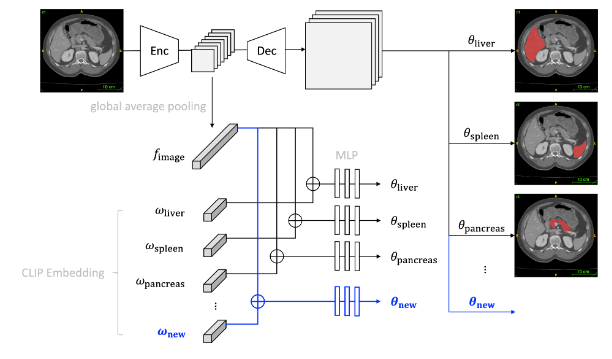
\includegraphics[width=\linewidth]{images/Cite-1-img1.png}
        \caption{An overview of image-aware organ-specific heads}
        \label{fig:Cite-1-img1}
    \end{figure}
        
    \textbf{Instruction tuning} In articles on Radiology-GPT and Radiology-LLAMA2 (both by Liu et al. \cite{cite-2}\cite{cite-3}) there was mention of instruction adjustment.
    Those two articles focus on the use of LLMs therefore, such technique was needed to keep the models focused on the task.
    In this particular example, Liu et al. used pairs of instructions "Findings —> Impression".  
    According to Rao et al. \cite{cite-4} prompt engineering such as this can be helpful in reducing the risk of hallucinations in LLMs.
    Similarly, by using specific prompts, it is possible to reduce defficencies in models complex reasoning.
    
    \textbf{Usage of Vicuina-13B}
    In their article Mukhrerjee et al.\cite{cite-23} used Vicuna language model to analyze chest radiograph (X-ray) reports for 13 different medical findings (e.g. atelectasis, cardiomegaly, pneumothorax). The goal was to classify each finding in the report as present (positive), absent (negative), uncertain, or not mentioned.
     
    The study used 13 predefined medical findings derived from CheXpert, a tool to label chest radiograph reports.
    Examples:
        \begin{itemize}
            \item Pathologic findings (e.g., pneumonia, lung opacity, pleural effusion)
            \item Support devices (e.g., pacemakers, tubes)
            \item The "no finding" label was excluded because it is automatically assigned if none of the other 12 pathologic findings are present.
        \end{itemize}
    Dependencies Between Labels
        \begin{itemize}
            \item Some findings imply others (e.g., cardiomegaly implies enlarged cardiomediastinum).
            \item Some findings (consolidation, edema, pneumonia) can imply lung opacity.
        \end{itemize}

    \textbf{DynaMMo} [17]
    
    \textbf{Modular networks for scanner/protocol adaptation} Another problem faced by continuous learning is heterogeneity in scanner hardware and imaging protocols.
    In their article, Rui et al.\cite{cite-19} propose a replay-based continuous learning (CL) framework with modular networks to solve these problems.
    Networks like those work by decomposing the models into task-specific sub-networks (modules).
    Then those modules can be dynamically combined or updated.
    In the case of medical imaging, the model would be divided into the following.
    \begin{itemize}
        \item Module for each scanner/protocol (e.g., Siemens MRI vs. GE CT)
        \item Shared backbone that extracts the general features from images (e.g., anatomical structures)
        \item Active learning module that selects the most informative samples to update modules.
    \end{itemize}
    Of course, a model like that would need components like: 
    \begin{itemize}
        \item Module Library: Stores protocol-specific modules (e.g., for T1 / T2 MRI, low-dose CT).
        \item Gating Mechanism: Routes input data to the relevant module based on metadata (e.g., scanner type) or learned features.
        \item Replay buffer: Retains exemplars of past protocols to mitigate forgetting.
    \end{itemize}
    This method works as follows.
    First, the input is analyzed.
    The scanner/protocol is detected either by reading metadata or by inferring it from image features.
    Next, the model selects the correct module.
    If the desired module already exists, it is simply activated, but if it does not, it is initialized and trained incrementally.
    The model then enters an active learning phase.
    In which the model queries the radiologist (oracle) to label ambiguous cases.
    In this step, only the affected module is updated, leaving others frozen.
    Finally, the model stores exemplars of past protocols to rehearse older knowledge.
    To save storage, this method uses coresets(compressed replay buffers).

    \textbf{Meta-Continual Learning: Combining meta-learning} 
    One way to mitigate catastrophic forgetting is Gradient Episodic Memory (GEM) proposed by Lopez-Paz \& Ranzato\cite{cite-30}.
    This method bridges meta-learning and continuous learning.
    Meta-learning (learning-to-learn) is a way to train model to quickly adapt to new task using very few examples.
    Gem achieves this by storing "memory" (episodic memory) of past tasks to constrain updates.
    And by optimizing gradients to avoid interference with prior knowledge.
    GEM works by:
    \begin{enumerate}
        \item Keeping the episodic memory.
        This method stores a subset of raw data (images and labels) in a fixed-size buffer.
        Unlike the more pure replay methods in GEM the episodic memory is used to guide the gradient updates not for retraining.
        \item Optimizing gradients.
        For each new task the GEM calculates its gradients ($\nabla L_{nev}$)
        Then it computes the gradients for past tasks using memory ($\nabla L_{old}$).
        Finally it projects ($\nabla L_{old}$) to avoid loss and ensure that the new updates do not harm performance of old tasks.
        It needs to solve a quadratic program to ensure 
        \[
           ( \nabla L_{old},\nabla L_{old} ) \geq 0
        \] 
        Gradient projection can be expressed as:
        \[
            \text{minimize}|| \nabla L_{nev} - v^2 ||\text{ s.t. } \langle v,\nabla L_{old} \rangle \geq 0
        \]
        \item Meta-Learning Aspect
        The projection step acts as a meta-learner, optimizing the direction of gradients to balance plasticity (new tasks) and stability (old tasks).
        Mimics MAML (Model-Agnostic Meta-Learning) in adapting to tasks efficiently, but tailored for CL.
    \end{enumerate}

    \textbf{CASA} Apart of catastrophic forgetting, while very pressing is not the only problem in continuous learning.
    In medicine (especially radiology), there exist a lot of hardware, imaging protocols, etc.
    To deal with heterogeneity of the data M. Perkonigg et al\cite{cite-10} proposed  continual active learning for scanner adaptation (CASA).
    This method assumes that there exists an oracle (in this case a radiologist) and that this oracle can return an accurate label for each image.
    However, queering an oracle is costly, so the goal of CASA is to train the network with a limited number of queries to the oracle while mitigating catastrophic forgetting.
    CASA achieves this by using pseudo-domains.
    Pseudo-domain is a group of images similar in some regard (its different from the direct domain because CASA assumes that we have no knowledge of scanner or protocol used).
    Additionally, CASA uses two memory modules, an outlier and training. 
    Outlier memory holds potential new pseudo-domains and the training one holds images for further training.
    CASA works as follows:
    \begin{enumerate}
        \item Model is pre-trained on labeled dataset for good initial performance
        \item From input stream model draws batch of unlabeled images.
        \item For each image, the pseudo-domain is calculated.
        \item The next step is decided on the basis of how well understood the pseudo-domain is. The image can be:\linebreak
        1. Added to labeled memory if the pseudo-domain it belongs to is still undertrained.\linebreak
        2. Added to the outlier memory if the style(pseudo-domain) is not recognized.\linebreak
        3. Discarded if the pseudo-domain is well understood.
    \end{enumerate}
        
    \begin{figure}
        \centering
        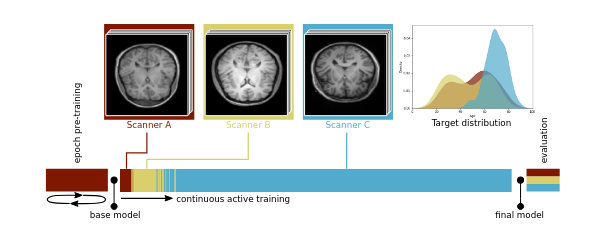
\includegraphics[width=\linewidth]{images/Cite-10-img-2.png}
        \caption{This is an experimental setup from M. Perkonigg et al\cite{cite-10}.
        First the model is pre-trainded on data from scanner A (red).
        Next the model is  gradually update with data from scanner B (yellow) then C (teal).
        Then the final model is evaluated on all 3 data sets. }
        \label{fig:Cite-10-img-2}
    \end{figure}
    \begin{figure}
        \centering
        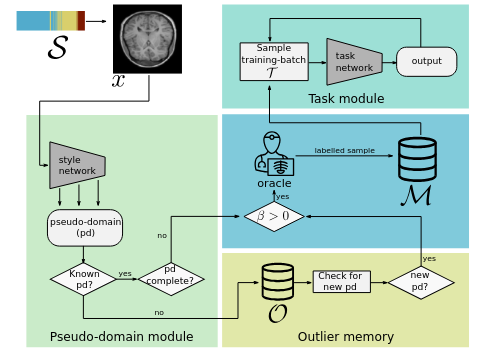
\includegraphics[width=\linewidth]{images/Cite-10-img-1.png}
        \caption{Overwiew of CASA algorithm\cite{cite-10}.}
        \label{fig:Cite-10-img-2b}
    \end{figure}
    \textbf{Reinforcement learning (RL)} In their work, Hu et al. discuss the evolution of deep Q-networks (DQN).
    From DQN itself to more advanced methods such as double DQN (DDQN), actor-critical (AC), A2C/A3C, and DDPG.
    These are algorithms used in medical image analysis, among other things.

    For reinforcement learning and its derivatives to work, they need a few key components:
    \begin{enumerate}
        \item Agent - the decision-maker or the learner
        \item Environment - The world for agent to interact with
        \item State (s) - state of environment
        \item Action (a)- Something agent can do
        \item Reward (r) - Feedback from environment
        \item Policy ($\pi$) - The strategy that maps actions to states
        \item Value Function - A way to estimate the result of taking action
    \end{enumerate}
    Typically, reinforcement learning works by:
    \begin{enumerate}
        \item Agent observation state (e.g., a chest X-ray).
        \item Select action (e.g., "diagnose pneumonia").
        \item The environment returns a reward (e.g., +1 if correct, -1 if wrong).
        \item The agent updates its policy to improve future decisions.
    \end{enumerate}
    In basic Q learning, the algorithm estimates the Q-value(expected reward) of taking an action in a state.
    \[
        Q(s,a) \leftarrow Q(s,a) + \alpha\left[r+\gamma max_{a'}Q(s',a') - Q(s,a)\right]
    \]
    \[
         \text{Where }\alpha = \text{learning rate,} \gamma = \text{discount factor}
    \]
    DQN improves on this method by:
    \begin{enumerate}
        \item Replacing table of Q values with approximates.
        \item Storing past transitions (s,a,r,s')(s,a,r,s') in a buffer and sampling minibatches to break correlations.
        \item Creating a second network, which slowly computes the values of Q
    \end{enumerate}
    Despite these advances, DQN still overestimates Q-values. 
    Therefore, there was the need to develop the methods discussed in the article that further improve upon DQN by:
    \begin{enumerate}
        \item Double DQN (DDQN) - Creating additional networks, one that selects the best action in the next state ($\theta$) and the other that calculates the Q value of the action chosen ($\theta^-$). In addition, the target function is updated to prevent the network from choosing over optimistic values.
        \[
            Y_t = r+\gamma Q(s',arg\space max_a'Q(s',a';\theta_t);\theta^-_t)
        \]
        \item Actor-Critic (AC) - Adding the policy gradients for actor and creating the critic. Output of the actor is updated using policy gradient theorem:
        \[
            \nabla J(\theta) = E[\nabla log\pi(a|s)Q(s,a)]
        \]
        And the critic evaluates the decision and provides the feedback to actor.
        \item A2C (Advantage Actor-Critic) \& A3C (Asynchronous A2C) - Sharing the policy gradient between parallel workers.
        A2C uses synchronous updates that can reduce variance.
        On the other hand, A3C uses asynchronous workers that work faster but can be less stable.
        \item DDPG (Deep Deterministic Policy Gradient) - Using deterministic actions.
        In this method, actor outputs deterministic actions is not  probabilistic, and Q-values are stored like in DQN.
        Additionally, this method stores transitions for stability.
    \end{enumerate}
    
    \begin{figure}
        \centering
        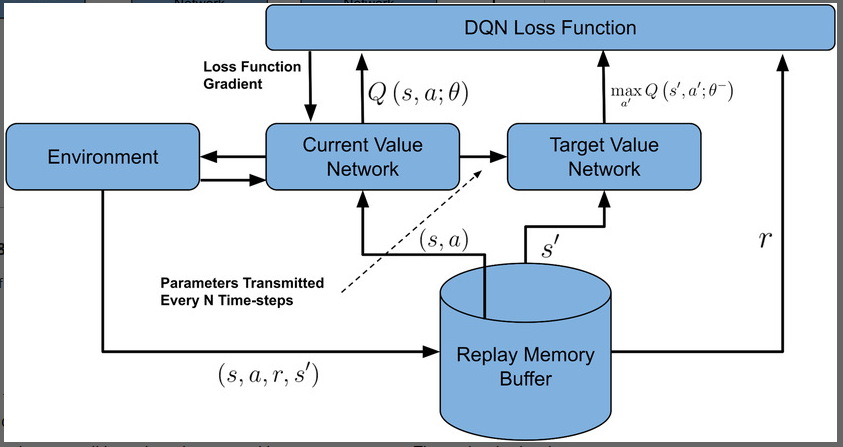
\includegraphics[width=\linewidth]{images/Cite-12-img-1.png}
        \caption{Approximate workflow for DQN.}
        \label{fig:enter-label}
    \end{figure}

    \textbf{Overlap Between RL and Continual Learning}
    While at first unrelated those two approaches deal with similar problems. 
    And can be used along side each other to enhance their outcomes.
    For example, Kaplanis et al. \cite{cite-31} in their article discuss the combination of CL and RL which can be called continual reinforcement learning (CRL).
    Traditionally, reinforcement learning struggles with agents that overwrite old knowledge when learning new tasks.
    That, of course, is catastrophic forgetting. 
    Therefore, using some techniques from continuous learning can be helpful in solving this problem.
    In this particular article, Kaplanis et al. use synaptic intelligence and integrate it with reinforcement learning.
    Synaptic intelligence is a continuous learning technique inspired by how the biological brain stores memories.
    Each synapse (neural network weight) is assigned the importance measure $\Omega$). 
    When the value of $\Omega$ is high, it means that the task is critical and should be protected from drastic changes.
    In the article, that technique was used in connection with DQN by:
    \begin{enumerate}
        \item Training DQN in Task 1.
        \item Computing synaptic importance for this task
        \item Training on task 2 while simultaneously penalizing the high $\Omega$ weights
    \end{enumerate}
    The loss function of this method can be expressed as:
    \[
        L = L_{RL} +\lambda \sum_i \Omega_i(\theta_i - \theta^*_i)^2
    \]
    Where:
    \[
       \theta^*_i \text{: Optimal weights for past tasks.}
    \]
    \[
        \lambda \text{: How strongly to protect old knowledge.}
    \]
    
    However, the tasks used in the article were simple Atari games for the model to play.
    However, combining those two techniques can prove useful in medical settings. 
    For example:
    \begin{itemize}
        \item An RL agent could learn new diseases (for example, COVID-19) without forgetting old ones (e.g., tuberculosis).
        \item Agents could adjust to new clinical guidelines while retaining prior decision-making skills.
        \item SI avoids expensive retraining from scratch.
    \end{itemize}
    \textbf{MUSCLE}
    In their article, Weibin et al.\cite{cite-17} proposed a new model training pipeline.
    This pipeline is supposed to deal with the heterogeneous data in enormous amounts.
    Their specific implementation focused on X-ray image analysis across many body parts (e.g., chest, bones) and tasks (e.g., segmentationm, detection).
    This method combines the following:
    \begin{itemize}
        \item Self-supervised learning (SSL) (MoCo framework) for representation learning.
        \item Continual learning (CL) to adapt to multiple tasks without catastrophic forgetting.
        \item Multitask / data set training to handle heterogeneous medical data. 
    \end{itemize}
    MUSCLE works in three main steps.
    \begin{enumerate}
        \item Multi-Dataset Momentum Contrastive Learning (MD-MoCo).
        In this step, the model learns a general representation from unlabeled X-ray images.
        For this to work properly, the images are resized to a constant resolution of 800x500 pixels.
        The grayscale distributions are then normalized using the Z score (mean = 122.786, std = 18.390).
        Finally, this step uses Momentum Contrast (MoCo) for SSL but disables augmentations like random cropping/blurring to preserve medical semantics
        \item Multi-Task Continual Learning (CL)
        Next step is to fine tune the backbone for diverse-tasks without forgetting previous knowledge.
        MUSCLE achieves this by using task-specific heads. 
        For example, Fully Connected Layer (FC) for classification (e.g., pneumonia detection), DeepLab-V3 for segmentation (e.g., lung masks) or Faster R-CNN for detection (e.g., tuberculosis)
        The training is split into 10 rounds, each iterating over the tasks sequentially. 
        Each task is trained for one epoch per round.
        The pipeline then uses regularization methods, such as elastic weight consolidation, to protect important weights.
        \item Task-Specific Fine-Tuning 
        Finally, the backbone is continuously adapted to individual tasks.
        This is achieved by freezing the backbone and fine-tuning the task-specific heads.
        \end{enumerate} 
    This pipeline shows a lot of promise in medical imaging.
    It can reduce the need to annotate the images.
    And can adapt to new tasks without the need to retrain the whole model.
    
    \textbf{RBACA Framework Architecture}
    The identified concerns with state-of-the-art replay-based methods have motivated the development of a novel continuous active learning framework called Replay-Based Architecture for Context Adaptation (RBACA)\cite{cite-19}.
    This framework addresses fundamental limitations in context representation quality through enhanced memory management and sample selection strategies\cite{cite-19}.
    RBACA employs a continuous learning memory-based rehearsal method integrated with an active learning component that selects informative instances based on uncertainty sampling and diversity considerations\cite{cite-19}.
    
    The RBACA architecture consists of four interconnected modules\cite{cite-19}: 
    \begin{itemize}
        \item the Pseudo-Context (PC) detection module, 
        \item memory-based rehearsal system, 
        \item active learning component, 
        \item incremental learning adaptation mechanism. 
    \end{itemize}
    The PC module evaluates each data stream sample, determining whether to route it to the oracle for annotation or to the outlier memory O through the active learning method. 
    When the outlier memory receives a new item, an evaluation process determines whether a new pseudo-context should be created and subsequently directed to the oracle for labeling\cite{cite-19}.
    The oracle labels and stores these instances in the rehearsal training memory $M$ of size $K_M$, which is utilized by the task module for network training as part of the continual learning component\cite{cite-19}.

    Memory Management and Pruning Strategies used in article are focused on implementing both static and dynamic allocation to maintain balanced representation among existing pseudo-contexts\cite{cite-19}. 
    In static memory management, when a new PC is identified, pruning is applied uniformly to all existing PCs to maintain memory balance\cite{cite-19}. 
    Conversely, dynamic memory management allocates $k$ new elements for each newly detected and annotated PC until maximum system memory capacity is reached\cite{cite-19}. 
    Both labeling budget $\beta$ and memory size $K_M$ influence the diversity of PCs in memory and the quality of their representations, with early consumption of $\beta$ potentially resulting in non-representation of later PCs in memory\cite{cite-19}.
   
    \paragraph{Metrics}
    One of the other challenges related to the use of artificial intelligence in radiology is the need for metrics to compare outputs. 
    The nature of machine learning requires continuous real-time monitoring for safe and reliable usage.
    This can be very impractical.
    Because that would require the input of the radiologist (which would be costly and inefficient).
    Therefore, there is a need for some metric to compare the quality of the model's prediction.
    
    \textbf{Predictive Divergence}
    In their article Venugopal et al.\cite{cite-7} proposed two main methods for comparing models and their outputs.
    \begin{enumerate}
        \item Predictive divergence is the measure of the quality of the main model's output.
        It consists of co-training other models along side the main one. 
        Then the output of the main model is compared with those of other models.
        Using divergence measures like Kullback-Leibler (KL) or Jensen-Shannon (JS), which will be explained later.
        In this method, the choice of secondary models is critical.
        They should complement main model's strengths and weaknesses.
        \item Temporal stability is the measure of the consistency of model's answers.
        The current prediction is compared with the averages of its historical prediction distributions.
    \end{enumerate}

    \textbf{Kullback-Leibler divergence}
        Kullback-Leibler divergence is a metric that quantifies how much one probability (P) distribution differs from the other (Q).
        It tells us how much data is lost when approximating the probability distribution P with Q.
        \[
            KL(P||Q) = \sum_x P(x)log\left(\frac{P(x)}{Q(x)}\right)
        \]
        The key properties of Kullback-Leibler divergence are as follows:
        \begin{enumerate}
            \item Asymmetry meaning that:
            \[
                KL(P||Q) \neq KL(Q||P)
            \]
            That's because it measures the divergence from Q to P, where P is the "true" distribution, and Q is the approximation 
            \item Non-negative
            \[
                KL(P||Q) \geq 0 
            \]
            \item Equal to 0 only if both Q and P are the same. And when the value grows, it means that the probabilities are more different from each other.
        \end{enumerate}
        
    \textbf{Jensen-Shannon divergence}
        Jensen-Shannon divergence is a measure of symmetric difference between two distributions (P and Q).
        It is based on Kullback-Leibler divergence but it fixes its asymetry.
        This metric can be expressed as:
        \[
            JS(P||Q) = \frac{1}{2}KL(P||Q) + \frac{1}{2}KL(Q||M)
        \]
        Where
        \[
            M = \frac{P+Q}{2}
        \]
        The key properties of Jensen-Shannon  divergence are as follows:
        \begin{enumerate}
            \item Symmetry meaning that unlike Kullback-Leibler:
             \[
                JS(P||Q) = JS(Q||P)
            \]
            \item Bounded values of Jensen-Shannon are between: 
            \[
                0 \leq JS(P||Q) \leq log(2)
            \]
            \item The same as Kullback-Leibler it is equal to 0 only if both Q and P are the same. And when the value grows, it means that the probabilities are more different from each other.
        \end{enumerate}

    \begin{figure}
        \centering
        \includegraphics[width=\linewidth]{images/Cite-19-img-1.png}
        \caption{Process of making a decision in RBACA}
        \label{fig:Cite-19-img-1}
    \end{figure}
    
    The framework addresses memory saturation concerns through sophisticated pruning techniques, including Least Recently Used (LRU) pruning for temporal-based sample removal, distribution-based methods such as K-Means clustering, Gaussian Mixture Models (GMMs), and Density-Based Spatial Clustering of Applications with Noise (DBSCAN)\cite{cite-19}.
    Additionally, informativeness-based techniques including Uncertainty Sampling and Expected Gradient Length (EGL) are employed, along with hybrid strategies that balance diversity and informativeness such as K-Means combined with Uncertainty Sampling (KU) and EGL combined with GMMs (EGL-GMM)\cite{cite-19}.
    
    Furthermore, the informativeness-based query method implements uncertainty sampling when new samples belong to known pseudo-contexts, utilizing a decision threshold to determine annotation necessity. 
    The uncertainty calculation for each sample is performed by inferring the unlabeled data pool through the task network, enabling efficient resource allocation within annotation budgets\cite{cite-19}.
    
    RBACA demonstrates adaptability for Class-Incremental Learning scenarios through dynamic architectural modifications. 
    The framework begins with a classification problem within a single episode, then leverages shared learned representations across episodes as the number of classes expands\cite{cite-19}.
    The most crucial adaptation occurs in the final layer of the task network, which initially starts with zero units and dynamically adds corresponding units when new classes are detected while preserving weights of previously identified classes\cite{cite-19}.
    
    The methodology builds upon the CASA architecture while implementing enhanced memory management, improved memory pruning strategies, more sophisticated identification of relevant samples, and expanded model capabilities for Class-IL scenarios.
    Although RBACA employs more complex techniques compared to CASA, this complexity is mitigated through parallelizable computational design .

    \textbf{IL-score as a benchmark metric}
    Rui et al. \cite{cite-19} have presented a novel approach in CAL benchmarking models, using a metric called incremental learning score (IL score).
    Given the lack of standardization of benchmarking tools to evaluate the performance of AI models, the authors suggested IL-score as a means to simultaneously assess the rate of transfer learning, forgetting, and overall model performance.
    For segmentation researchers used, the Dice Similarity Coefficient (DSC) to assess agreement between prediction and target.
    Alternatively, they proposed to use the F1 Score, calculated as the arithmetic mean of the per-class metric.
    To assess forgetting they used Backward Transfer (BWT) \cite{cite-30}, which measures how learning a new context affects performance on previously learned contexts\cite{cite-19}.
    BWT is defined as
    $$
    \mathrm{BWT} =\frac{1}{t-1} \sum_{j=1}^{t-1} (a_{t,j} - a_{j,j})
    $$
    where $a_{x,y}$ shows the test metric (DSC) for context $y$ after learning from context $x$.
    In this formula $t$ is the final learned context.
    As the metric used to measure the impact of prior context on the performance of the new, the converse formula - Forward Transfer (FWT), given by
    $$
    \mathrm{FWT} = \frac{1}{t-1} \sum_{j=2}^{t} \left( a_{j-1,j} - \overline{b}_j \right)
    $$
    Here $\overline{b}_j$ denotes the test metric for context $j$ at random initialization.
    DSC and F1 score give a result in the range [0,1], BWT gives a result in the range [-1,1], and finally FWT gives a score in the range [-1,1].
    After calculating an average of these metrics, we obtain the IL-Score, ranging from [-2/3, 1], where higher values indicate superior performance\cite{cite-19}. 
    
    \textbf{PACS/RIS integration} For artificial intelligence to provide the most benefits to actual radiologists, it must be properly integrated into their workflow.
    In their article, Srivastava et al.\cite{cite-6} propose a framework for doing exactly that.
    This is done by directly integrating artificial intelligence assistants into radiation information systems (RIS) and picture archiving and communication systems (PACS).
    Real-Time Image Analysis

    For the integration of artificial intelligence to be seamless, this specific method implements the following.
    \begin{enumerate}
        \item DICOM Image Processing: The artificial intelligence model pulls images from PACS, processes them (for example, tumor segmentation), and pushes back annotations or structured reports.
        For example, the model detects lung nodules on CT scans and inserts findings into RIS.
        \item Workflow automation: The images are analyzed.
        The model can then prioritize urgent cases (e.g., pneumothorax) in the radiology work list based on the impression of the images.
        \item Report Generation: The artificial intelligence model drafts impressions from findings (e.g., "8mm pulmonary nodule, recommend follow-up in 3 months").
        The model is capable of natural language processing.
        Based on the findings, model can prepare draft of the report.
        The model supports multilingual reports for global clinics.
        \item Query handling: Radiologists ask AI questions (e.g., "Show similar cases with biopsy-proven malignancy").
        \item Human-in-the-Loop (HITL): Radiologists edit AI-generated reports.
        Corrections train the model continuously.
        \item Bias mitigation: Tracks AI errors (e.g., over diagnosis of nodules) and adjusts confidence thresholds.
    \end{enumerate}
    
    \textbf{Human-in-the-Loop (HITL) Systems}
        Human-in-the-Loop (HITL) refers to systems where human expertise is integrated into machine learning (ML) processes to improve model performance, particularly in uncertain or evolving environments.
        Konyushkova et al.\cite{cite-10} explore this in the context of Continual Active Learning (CAL) for adapting ML models to changing data distributions (e.g., medical imaging with varying acquisition conditions).
        In this context, the model uses active learning to select data points that will be most valuable to label.
        The paper emphasizes selecting the "most valuable" samples for human labeling. Common strategies include:
            \begin{itemize}
                \item Uncertainty Sampling: Query samples where the model’s prediction entropy is highest.
                \item Diversity Sampling: Ensure selected samples cover diverse feature spaces.
                \item Committee-Based (Query-by-Committee): Use multiple models; label samples with the highest disagreement.
            \end{itemize}
        For example: In medical imaging, the model might prioritize ambiguous tumor boundaries for expert review.
 
        Human expert labels the chosen images, thus ensuring efficient adaptation.
        Then the continuous learning takes place, and the model is retrained on newly labeled data.
        This, of course, is done with proper steps to avoid catastrophic forgetting.
               
        The paper likely uses techniques like:
            \begin{itemize}
                \item Elastic Weight Consolidation (EWC): Penalizes changes to weights critical for past tasks.
                \item Replay Buffers: Stores and revisits old labeled samples during retraining.
                \item Regularization: Constraints model updates to preserve prior knowledge.
            \end{itemize}
        Thanks to this combination of features, the method provides benefits like:
        \begin{itemize}
            \item Efficiency: Reduces annotation costs by only querying the most useful samples.
            \item Adaptability: Helps models stay accurate as data evolves (e.g., new medical scanners).
            \item Robustness: Human expertise corrects model biases and errors.
        \end{itemize}
        
\section{METHODS}

    \subsection{Methods used in related works}

    \subsubsection{MUSCLE Framework Architecture}    
    \textbf{Three-Phase Methodological Approach}
    MUSCLE employs a systematic three-phase approach that distinguishes it from conventional self-supervised learning methods in medical imaging\cite{cite-17}.
    The framework consists of:
    \begin{itemize}
        \item Multi-Dataset Momentum Contrastive Learning (MD-MoCo), 
        \item Multi-Task Continual Learning,
        \item Fine-tuning on Downstream Tasks
    \end{itemize}
    This represents a comprehensive pipeline for X-ray image analysis. 
    This methodological structure enables the framework to aggregate X-rays collected from multiple body parts for MoCo-based representation learning, while adopting a well-designed continual learning procedure to further pre-train the backbone for various X-ray analysis tasks jointly\cite{cite-17}.


    \begin{figure}
        \centering
        \includegraphics[width=\linewidth]{images/Cite-17-img-1.png}
        \caption{Process of making a decision in RBACA}
        \label{fig:Cite-17-img-1}
    \end{figure}
    
    \textbf{Multi-Dataset Momentum Contrastive Learning (MD-MoCo) Methodology}\newline
    The first methodological component addresses the fundamental challenge of data heterogeneity across multiple X-ray datasets through sophisticated preprocessing and normalization strategies. 
    MUSCLE collects and aggregates nine X-ray image datasets, offering nearly 179,000 X-ray images covering several parts of the human body\cite{cite-17}, including:
    \begin{itemize}
        \item chest
        \item hand
        \item forearm
        \item humerus
        \item and others.
    \end{itemize}
    
    To address these challenges, MUSCLE implements systematic preprocessing schemes that transform and normalize the grayscale distribution using the Z-score method with a mean of 122.786 and a standard deviation of 18.390.
    The framework resizes all images to 800×500 resolution,which balances effectiveness and efficiency of deep learning while fully utilizing GPU resources for the resource-consuming MoCo algorithms. 
    Additionally, MUSCLE extends MoCo-CXR with advanced settings on data augmentation strategies and initialization tricks, specifically disabling random cropping, Gaussian blurring, and color / grayscale jitter to preserve semantic information for medical images\cite{cite-17}.
    
    \textbf{Multi-Task Continual Learning Implementation}\\
    The second methodological phase employs sophisticated continual learning strategies to address catastrophic forgetting through task-specific head architectures and regularization mechanisms. 
    MUSCLE extends vanilla continual learning for neural networks by iterating training procedures of the backbone network with alternating task-specific heads, including Fully Connected layers for classification tasks, DeepLab-V3 for segmentation tasks, and FasterRCNN for detection tasks\cite{cite-17}. 
    The framework splits the continuous learning procedure into 10 rounds of the learning process, where each round iterates through 4 learning tasks one by one, with each iteration training the backbone network for 1 epoch using a task-specific head\cite{cite-17}.
    
    To avoid overfitting to any single task, MUSCLE implements a cyclic and reshuffled learning schedule that reshuffles the order of tasks in every round of the learning process and adopts a Cosine annealing learning rate schedule\cite{cite-17}. 
    The framework also employs cross-task memorization with explicit bias to address catastrophic forgetting, leveraging knowledge transfer regularization derived from L2-SP that constrains the distance between learning outcomes and the backbone trained by previous iterations\cite{cite-17}.
    
    \textbf{Fine-Tuning Methodology for Downstream Tasks}\\
    The final phase of MUSCLE employs task-specific fine-tuning strategies that connect the pre-trained backbone with appropriate task-specific heads for independent and separate adaptation.
    The framework fine-tunes the backbone on each of the four tasks independently, connecting the pre-trained backbone with Fully Connected layers for classification tasks, DeepLab-V3 for segmentation tasks, and FasterRCNN for detection tasks\cite{cite-17}. MUSCLE employs standard settings such as vanilla weight decay as stability regularization and step-based decay of learning rate schedule for fine-tuning processes\cite{cite-17}.
    
    \textbf{Experimental Validation and Performance Assessment}\\
    The MUSCLE framework has been evaluated using comprehensive experimental protocols across nine real-world X-ray datasets with various tasks like:
    \begin{itemize}
        \item pneumonia classification
        \item skeletal abnormality classification
        \item lung segmentation
        \item tuberculosis detection
    \end{itemize} 
    Comparisons against other pre-trained models confirm the proof-of-concept that self-supervised multitask / dataset continual pre-training can boost the performance of X-ray image analysis\cite{cite-17}. 
    The framework demonstrates superior performance over ImageNet and MoCo pre-trained backbones using both ResNet-18 and ResNet-50 as backbone architectures, with results showing significant improvements in accuracy, sensitivity, specificity, and AUC across multiple medical imaging tasks.
    
    \textbf{Integration with Broader Continual Learning Literature}\\
    The methodological contributions of MUSCLE align with broader trends in continual learning for medical imaging, where frameworks address the dynamic nature of healthcare data and the need for models that can adapt to new contexts without forgetting previously learned knowledge\cite{cite-18}.
    The framework approach to multi-dataset aggregation and task-specific head architectures represents an advancement in addressing data heterogeneity challenges commonly encountered in medical imaging applications\cite{cite-17}. 
    MUSCLE's integration of self-supervised learning with continual learning paradigms demonstrates the potential for developing more robust and adaptable AI systems for medical image analysis, contributing to the growing body of literature on continual learning applications in healthcare\cite{cite-27}.



    \subsubsection{RBACA Framework Architecture} 
    
    \textbf{Continual Active Learning Integration}\\
    The Replay-Based Architecture for Context Adaptation (RBACA) introduces a novel continual active learning (CAL) framework that addresses fundamental limitations in medical imaging through enhanced memory management and active learning integration\cite{cite-19}.
    The framework consists of four interconnected components:
    \begin{itemize}
        \item Pseudo-Context (PC) Detection Module
        \item Memory-Based Rehearsal System  
        \item Active Learning Component
        \item Incremental Learning Adaptation Mechanism
    \end{itemize}
    This integration represents a significant advancement in medical imaging adaptation by addressing both knowledge retention and annotation efficiency challenges simultaneously\cite{cite-19}.
    
    \textbf{Pseudo-Context Detection and Memory Management}\\
    The RBACA framework implements automatic recognition of shifts in image characteristics through sophisticated context identification mechanisms that do not require explicit domain labels.
    The Pseudo-Context (PC) module evaluates each data stream sample, determining whether to route it to the oracle for annotation or to the outlier memory through the active learning method\cite{cite-19}.
    When the outlier memory receives a new item, an evaluation process determines whether a new pseudo-context should be created and subsequently directed to the oracle for labeling.
    
    RBACA employs advanced memory management strategies including both static and dynamic allocation approaches to maintain balanced representation among existing pseudo-contexts\cite{cite-19}.
    In static memory management, when a new PC is identified, pruning is applied uniformly to all existing PCs to maintain memory balance.
    Conversely, dynamic memory management allocates $k$ new elements for each newly detected and annotated PC until maximum system memory capacity is reached.
    Both labeling budget $\beta$ and memory size $K_M$ influence the diversity of PCs in memory and the quality of their representations, with early consumption of $\beta$ potentially resulting in non-representation of later PCs in memory\cite{cite-19}.
    
    \textbf{Memory Pruning Strategies and Techniques}\newline
    The framework addresses memory saturation concerns through sophisticated pruning techniques that balance representativeness and computational efficiency.
    RBACA implements multiple pruning methodologies including Least Recently Used (LRU) for temporal-based sample removal, distribution-based methods such as K-Means clustering, Gaussian Mixture Models (GMMs), and Density-Based Spatial Clustering of Applications with Noise (DBSCAN)\cite{cite-19}.
    
    Additionally, informativeness-based techniques including Uncertainty Sampling and Expected Gradient Length (EGL) are employed to select the most valuable samples for retention.
    The framework also supports hybrid strategies that balance diversity and informativeness, such as K-Means combined with Uncertainty Sampling (KU) and EGL combined with GMMs (EGL-GMM)\cite{cite-19}.
    In these hybrid approaches, clustering is first applied, and for each cluster $i$, $k_i$ samples are selected: the $k_i/2$ closest to the centroid, and among the remaining samples, the $k_i/2$ most informative.
    
    \textbf{Active Learning Integration and Query Strategy}\newline
    The informativeness-based query method implements uncertainty sampling when new samples belong to known pseudo-contexts, utilizing a decision threshold to determine annotation necessity\cite{cite-19}.
    The uncertainty calculation for each sample is performed by inferring the unlabeled data pool through the task network, enabling efficient resource allocation within annotation budgets.
    This approach ensures that the most informative instances are selected for annotation while maintaining diversity in the training data.
    
    RBACA enables an uncertainty sampling strategy based on informativeness, using a decision threshold to make annotation decisions.
    When a new sample belongs to a known PC, the active learning algorithm must determine whether to annotate or discard the instance, optimizing the use of limited labeling resources\cite{cite-19}.
    
    \textbf{Adaptation to Class-Incremental Learning}\newline
    RBACA demonstrates remarkable adaptability for Class-Incremental Learning (Class-IL) scenarios through dynamic architectural modifications that preserve previously learned knowledge while accommodating new classes\cite{cite-19}.
    The framework begins with a classification problem within a single episode, then leverages shared learned representations across episodes as the number of classes expands.
    
    The most crucial adaptation occurs in the final layer of the task network, which initially starts with zero units and dynamically adds corresponding units when new classes are detected while preserving weights of previously identified classes\cite{cite-19}.
    This adaptation involved modifications in the data loading phase, the task network model, and the evaluation metrics, ensuring that RBACA is adaptable to any classification problem where the number of classes is not predefined and new classes may emerge over time.
    
    \textbf{IL-Score Evaluation Methodology}\newline
    RBACA introduces the Incremental Learning Score (IL-Score) as a comprehensive evaluation metric that simultaneously assesses transfer learning capabilities, catastrophic forgetting mitigation, and overall model performance across all learned contexts\cite{cite-19}.
    This novel metric represents a significant advancement in continual learning evaluation for medical imaging applications, providing a unified framework for assessing the effectiveness of continual active learning methods.
    
    The IL-Score enables simultaneous assessment of three critical aspects: knowledge transfer from previous contexts, retention of previously learned information, and final model performance across diverse medical imaging scenarios\cite{cite-19}.
    This comprehensive evaluation approach allows for more robust comparison of different continual learning strategies and provides insights into the trade-offs between plasticity and stability in medical imaging applications.
    
    \textbf{Experimental Validation and Performance Assessment}\newline
    The RBACA framework has been rigorously evaluated using comprehensive experimental protocols in both domain-incremental and class-incremental learning scenarios through cardiac image segmentation and diagnosis tasks\cite{cite-19}.
    The framework demonstrates superior performance compared to baseline methods without CAL and state-of-the-art approaches such as CASA across various memory sizes and annotation budgets.
    
    Experimental results show that RBACA outperforms both a baseline framework without CAL (SeqFineTune) and the CASA method across multiple configurations, demonstrating its adaptability and effectiveness in medical imaging contexts\cite{cite-19}.
    The evaluation encompassed various memory management strategies, pruning techniques, and active learning configurations, providing comprehensive evidence of RBACA's robustness and versatility.
    
    \textbf{Integration with Broader Continual Learning Literature}\newline
    RBACA's methodological contributions align with broader trends in continual learning for medical imaging, where frameworks address the dynamic nature of healthcare data and the need for models that can adapt to new contexts without forgetting previously learned knowledge\cite{cite-18}.
    The framework's approach to memory management and active learning integration represents an advancement in addressing both catastrophic forgetting and annotation efficiency challenges commonly encountered in medical imaging applications\cite{cite-19}.
    
    RBACA's integration of continual learning with active learning paradigms demonstrates the potential for developing more robust and efficient AI systems for medical image analysis, contributing to the growing body of literature on continual learning applications in healthcare\cite{cite-27}.
    The framework establishes important benchmarks for future research in continual active learning applications for radiology and medical image analysis.

\section{Conclusion}

    The development of AI models in radiology through continuous learning represents a transformative shift in medical imaging, offering solutions to dynamic data challenges while introducing novel methodological frameworks. 
    This article synthesizes key advancements in architectures, training paradigms, and evaluation metrics, highlighting both the promise and persisting hurdles in deploying these systems clinically.
    
    \subsection{Key Advancements}
    Continuous learning frameworks like \textbf{MUSCLE} (multi-task self-supervised learning) \cite{cite-17} and \textbf{RBACA} (replay-based active learning) \cite{cite-19} demonstrate robust strategies for mitigating catastrophic forgetting and adapting to domain shifts in radiology workflows. 
    These methods leverage hybrid approaches—combining regularization, replay, and dynamic model expansion—to balance plasticity and stability. 
    For instance, MUSCLE’s integration of momentum contrastive learning with task-specific heads enables effective multi-dataset aggregation across diverse anatomical regions \cite{cite-17}, while RBACA’s pseudo-context detection and memory pruning strategies optimize annotation efficiency in evolving clinical environments \cite{cite-19}. 
    Theoretical contributions, such as the \textbf{IL-Score} \cite{cite-19}, provide comprehensive metrics for assessing transfer learning, forgetting, and model capacity, addressing the critical need for standardized benchmarks.
    
    \subsection{Persistent Challenges}
    Despite progress, several issues merit attention:
    
    1. \textbf{Standardization Gaps}: The lack of unified datasets and evaluation protocols hinders direct comparison of models. 
    While studies like Yixiao et al. \cite{cite-1} validate continuous learning on independent test sets, most frameworks rely on institution-specific data, limiting generalizability.
    
    2. \textbf{Ethical and Computational Trade-offs}: Replay-based methods \cite{cite-19}, though effective, raise privacy concerns due to raw data storage. 
    Hybrid techniques, while balancing performance, increase computational complexity \cite{cite-10}, posing barriers to real-time clinical integration.
    
    3. \textbf{Longitudinal Validation}: Many studies, including the breast MRI analysis by Hui et al. \cite{cite-21}, use retrospective data. 
    Prospective validation across diverse populations and imaging protocols is needed to assess long-term efficacy and model decay.
    
    4. \textbf{Human-AI Collaboration}: While systems like \textbf{LibreHealth RIS} \cite{cite-6} embed AI into radiologist workflows, automation bias remains a risk. 
    Human-in-the-loop mechanisms must be refined to ensure radiologists retain oversight, particularly when models generate pseudo-labels or prioritize studies.
    
    \subsection{Future Directions}
    1. \textbf{Swarm Learning and Decentralized Frameworks}: Platforms enabling multi-institutional collaboration without raw data sharing—e.g., weight-based updates in federated learning \cite{cite-6}—could address privacy concerns while enhancing model robustness.
    
    2. \textbf{Dynamic Adaptation to Emerging Data}: Integrating real-time detection of scanner/protocol shifts (as in \textbf{CASA} \cite{cite-10}) with automated model updates will be critical as imaging technologies evolve.
    
    3. \textbf{Education and Competency Development}: As shown by Verhoeven et al. \cite{cite-8}, radiology curricula must evolve to include AI stewardship, ensuring practitioners can audit models and mitigate biases introduced during continuous learning.
    
    In conclusion, continuous learning paradigms hold immense potential to revolutionize radiology AI, but their success hinges on addressing standardization, ethical, and translational challenges. Collaborative efforts among clinicians, engineers, and policymakers will be essential to navigate these complexities and realize the full promise of adaptive AI in healthcare.
    

\begin{thebibliography}{31}
    \bibitem{cite-1}  
    Yixiao Zhang, Xinyi Li, Huimiao Chen, Alan Yuille, Yaoyao Liu, \& Zongwei Zhou. (2023).
    \textit{Continual Learning for Abdominal Multi-Organ and Tumor Segmentation.}
    arXiv. \url{https://arxiv.org/abs/2306.00988}
    \bibitem{cite-2}  
        Zhou, Z., Lyu, Q., Tang, Y., Han, Z., Chen, J., \& Wang, S. (2023). \textit{Radiology-GPT: A large language model for radiology}. arXiv. \url{https://arxiv.org/abs/2306.08666}
    \bibitem{cite-3}  
        Zhou, Z., Lyu, Q., Tang, Y., Han, Z., Chen, J., \& Wang, S. (2023). \textit{Radiology-Llama2: Best-in-class large language model for radiology}. arXiv. \url{https://arxiv.org/abs/2309.06419}
    \bibitem{cite-4} 
        Nguyen, D. Q., Nguyen, T. T., Dao, T. H., Duong, Q. H., Vu, X. H., Pham, H. H., Nguyen, H. Q., \& Nguyen, H. (2024). \textit{CheX-GPT: Harnessing large language models for enhanced chest X-ray report labeling}. arXiv. \url{https://arxiv.org/abs/2401.11505}
    \bibitem{cite-5}
        Rao, A., Kim, S., Kamineni, M., Pang, B., Lie, W., \& Lungren, M. P. (2023). \textit{Chatbots and large language models in radiology: A practical primer for clinical and research applications}. Radiology, 310(2), e232756. \url{https://doi.org/10.1148/radiol.232756}
    \bibitem{cite-6}  
        Srivastava, R., Ma, X., \& Lakhani, P. (2023).\textit{ A general-purpose AI assistant embedded in an open-source radiology information system}. arXiv. \url{https://arxiv.org/abs/2303.10338}
    \bibitem{cite-7} 
        Srivastava, R., Ma, X., \& Lakhani, P. (2023). \textit{New epochs in AI supervision: Design and implementation of an autonomous radiology AI monitoring system}. arXiv. \url{https://arxiv.org/abs/2311.14305}
    \bibitem{cite-8}
        Verhoeven, M., Deroo, M., \& Semaille, P. (2023). \textit{A framework to integrate artificial intelligence training into radiology residency programs: Preparing the future radiologist}. Insights into Imaging, 14, 132. \url{https://doi.org/10.1186/s13244-023-01595-3}
    \bibitem{cite-9}
        Lungren, M. P., et al. (2024).\textit{Development and external validation of an artificial intelligence model for identifying radiology reports containing recommendations for additional imaging}. American Journal of Roentgenology. \url{https://doi.org/10.2214/AJR.23.29120}
    \bibitem{cite-10}
        Konyushkova, K., Sznitman, R., \& Fua, P. (2021). \textit{Continual active learning for efficient adaptation of machine learning models to changing image acquisition}. arXiv. \url{https://arxiv.org/abs/2106.03351}
    \bibitem{cite-11}
        Wang, J., Chen, M., Zhang, Y., Zhao, Y., \& Liu, J. (2023). \textit{Continual learning in medical image analysis: A comprehensive review of recent advancements and future prospects}. arXiv. \url{https://arxiv.org/abs/2312.17004}
    \bibitem{cite-12}
        Chen, D., Yang, G., Xu, L., \& Wang, T. (2024). \textit{Reinforcement learning in medical image analysis: Concepts, applications, challenges, and future directions}. Journal of Applied Clinical Medical Physics. \url{https://doi.org/10.1002/acm2.13898}
    \bibitem{cite-13}
        Langlotz, C. P., Allen, B., Erickson, B. J., Kalpathy-Cramer, J., Bigelow, K., Cook, T. S., ... \& Dreyer, K. (2019). \textit{Artificial intelligence and machine learning in radiology: Opportunities, challenges, pitfalls, and criteria for success}. Journal of the American College of Radiology, 16(4), 504–510. \url{https://doi.org/10.1016/j.jacr.2018.09.019}
    \bibitem{cite-14}
        Hosny, A., Parmar, C., Quackenbush, J., Schwartz, L. H., \& Aerts, H. J. W. L. (2018). \textit{Machine learning: Applications of artificial intelligence to imaging and diagnosis}. Nature Reviews Cancer, 18, 500–510. \url{https://pmc.ncbi.nlm.nih.gov/articles/PMC10248832/}
    \bibitem{cite-15}
        Mirniaharikandehei, S., Hames, T. K., \& Greenspan, H. (2023). \textit{Overcoming diagnostic challenges of artificial intelligence in pathology and radiology: Innovative solutions and strategies}. International Journal of Medical Students, \textit{11}(3), 107--113. \url{https://pmc.ncbi.nlm.nih.gov/articles/PMC10248832/}
    \bibitem{cite-16}
        Lakhani, P., \& Sundaram, B. (2017). \textit{Machine learning in radiology: Applications beyond image interpretation}. Journal of the American College of Radiology, \textit{14}(4), 541--546. \url{https://cerf.radiologie.fr/sites/cerf.radiologie.fr/files/Enseignement/pdf/Machine%20Learning%20in%20Radiology%20Applications%20Beyond%20Image%20Interpretation_Lakhani_JACR%202017.pdf}
    \bibitem{cite-17}
        Weibin Liao, Haoyi Xiong, Qingzhong Wang, Yan Mo, Xuhong Li, Yi Liu, Zeyu Chen, Siyu Huang, Dejing Dou. 
        \textit{MUSCLE: Multi-task Self-supervised Continual Learning to Pre-train Deep Models for X-ray Images of Multiple Body Parts}
        arXiv. \url{https://arxiv.org/abs/2310.02000}
    \bibitem{cite-18}
        Kumar, A., Aggarwal, A., Joshi, A., Bhargava, H., \& Patra, B. K. (2024). \textit{Continual learning in medical imaging: A survey and practical analysis}. arXiv. \url{https://arxiv.org/abs/2405.13482}
    \bibitem{cite-19}   
        Rui Daniel, M. Rita Verdelho, Catarina Barata, \& Carlos Santiago. (2025). 
        \textit{Continual Deep Active Learning for Medical Imaging: Replay-Base Architecture for Context Adaptation.}
        . arXiv. \url{https://arxiv.org/abs/2501.08245}
    \bibitem{cite-20}
        Hosny, A., Parmar, C., Quackenbush, J., Schwartz, L. H., \& Aerts, H. J. W. L. (2018). \textit{Deep learning workflow in radiology: A primer}. Insights into Imaging, 9, 1--11. \url{https://doi.org/10.1186/s13244-019-0832-5}
    \bibitem{cite-21}
        Li H, Whitney HM, Ji Y, et al. 
        \textit{Impact of continuous learning on diagnostic breast MRI AI: evaluation on an independent clinical dataset.}
        J Med Imaging (Bellingham). 2022;9(3):034502. doi:10.1117/1.JMI.9.3.034502
        \url{https://pmc.ncbi.nlm.nih.gov/articles/PMC9168763/}
    \bibitem{cite-22}
        Nguyen, D. Q., Nguyen, T. T., Dao, T. H., Duong, Q. H., Vu, X. H., Pham, H. H., Nguyen, H. Q., \& Nguyen, H. (2024). \textit{CheX-GPT: Harnessing large language models for enhanced chest X-ray report labeling}. arXiv. \url{https://arxiv.org/abs/2401.11505}
    \bibitem{cite-23}
        Pritam Mukherjee, Benjamin Hou, Ricardo B. Lanfredi, Ronald M. Summers \textit{Feasibility of Using the Privacy-preserving Large Language Model Vicuna for Labeling Radiology Reports}. \url{https://pubs.rsna.org/doi/10.1148/radiol.231147}
    \bibitem{cite-24}  
        Jacob Devlin, Ming-Wei Chang, Kenton Lee, and Kristina Toutanova. \textit{Bert: Pre training of deep bidirectional transformers for language understanding}. arXiv. \url{https://arxiv.org/pdf/1810.04805}  
    \bibitem{cite-25}  
       Carrodeguas E, Lacson R, Swanson W, Khorasani R. Use of Machine Learning to Identify Follow-Up Recommendations in Radiology Reports. \url{https://pmc.ncbi.nlm.nih.gov/articles/PMC7534384/}
    \bibitem{cite-26}
    Guangyao Zheng, Samson Zhou, Vladimir Braverman, Michael A Jacobs,and Vishwa Sanjay Parekh, “Selective experience replay compression using coresets for lifelong deep reinforcement learning in medical imaging,” in Medical Imaging with Deep Learning. PMLR, 2024, pp. 1751–1764.\url{https://arxiv.org/abs/2302.11510}
    \bibitem{cite-27}
    Mohammad Areeb Qazi, Anees Ur Rehman Hashmi, Santosh Sanjeev, Ibrahim Almakky, Numan Saeed, Camila Gonzalez, Mohammad Yaqub Continual Learning in Medical Imaging: A Survey and Practical Analysis\url{https://arxiv.org/abs/2405.13482}
    \bibitem{cite-28}
    Wade, Stuart W T et al. “What works in radiology education for medical students: a systematic review and meta-analysis.” BMC medical education vol. 24,1 51. 10 Jan. 2024, doi:10.1186/s12909-023-04981-z \url{https://pmc.ncbi.nlm.nih.gov/articles/PMC10782640/}
    \bibitem{cite-29}
    Harthoorn, Frederike S et al. \textit{“Radiology education for medical students: a qualitative exploration of educational topics, teaching methods and future strategies.”} BMC medical education vol. 24,1 891. 19 Aug. 2024, doi:10.1186/s12909-024-05879-0\url{https://pmc.ncbi.nlm.nih.gov/articles/PMC11334451/}
    \bibitem{cite-30}
    David Lopez-Paz and Marc’Aurelio Ranzato, \textit{“Gradient episodic memory for continual learning,” Advances in Neural Information Processing}
    Systems, vol. 30, 2017. \url{https://arxiv.org/abs/1706.08840}
    \bibitem{cite-31}
    Christos Kaplanis,Murray Shanahan,Claudia Clopath \textit{Continual Reinforcement Learning with Complex Synapses}.\url{https://arxiv.org/pdf/1802.07239}
    \bibitem{cite-32}
    Seyed Iman Mirzadeh, Mehrdad Farajtabar, Dilan Gorur, Razvan Pascanu, Hassan Ghasemzadeh \textit{Linear Mode Connectivity in Multitask and Continual Learning} \url{https://arxiv.org/pdf/1802.07239}
\end{thebibliography}\vspace*{-8pt}

\end{document}

